\documentclass{article}
\usepackage[T1]{fontenc}
\usepackage{lmodern}
\usepackage{graphicx}
\usepackage{amsmath,amssymb}
\usepackage[a4paper,margin=2cm]{geometry}
\usepackage[absolute,overlay]{textpos}
\setlength{\TPHorizModule}{1mm}
\setlength{\TPVertModule}{1mm}
\usepackage[indonesian]{babel}
\usepackage{hyperref}
\setlength{\emergencystretch}{2em}
% unit: Halaman 15

\begin{document}

% === Halaman 15 (llm) ===

% (tidak ada teks dari model)

% deskripsi: Screenshot Command Prompt yang menunjukkan proses enkripsi dan dekripsi file teks menggunakan program enkrip_xor dan dekrip_xor dengan kata kunci 'viruscorona'.
% bbox normalisasi: [0.0650, 0.2010, 0.9350, 0.8140]
\begin{textblock*}{182.70mm}(13.65mm,59.70mm)
\noindent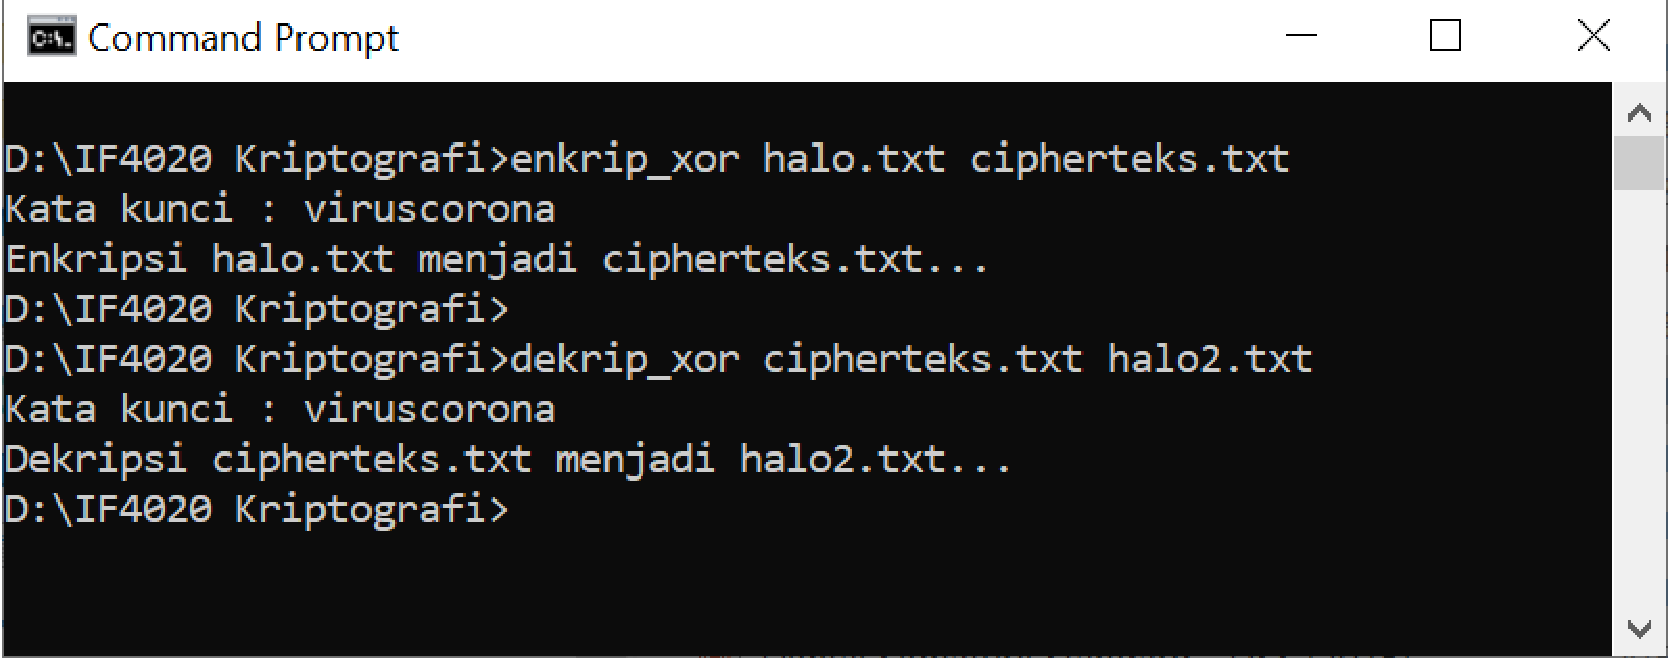
\includegraphics[width=182.70mm,height=182.06mm]{../../images/llm/page_015_img_01.png}%
\end{textblock*}

\end{document}
